\section{Auswertung}
\subsection{Vorgehen und genutzte Programme}
Zur Automatisierung der Auswertung wird wie folgt vorgegangen:
\begin{enumerate}
  \item Die Filme werden auf einem Scanner digitalisiert.
  Der Film der Salzprobe muss dabei während des scannens von oben beleuchtet werden,
  da der Film durch die längere Messdauer und Streulicht sehr stark belichtet
  wurde.
  \item Die gescannten Bilder werden digital nachbearbeitet, sodass die
  Beugungskreise besser hervortreten.
  \item Zwischen den Stanzungen der Filme werden die Grauwerte in einem schmalen,
  mittigen Streifen ausgelesen.
  Dazu wird das Programm ImageJ\cite{Schneider2012} genutzt.
  \item Die Grauwerte werden in einem Python\cite{python}-script
  durch Pandas\cite{mckinney-proc-scipy-2010} eingelesen.
  Der Grauwert wird invertiert und der Untergrund manuell auf ein
  einheitliches Niveau zu heben.
  \item Durch die Funktion \texttt{find\_peaks} der SciPy\cite{scipy}-Bibliothek
  \texttt{signal} werden die Peaks und damit die Beugungskreise detektiert.
  Die Abstände zum Mittelpunkt der Stanzung in Millimeter entsprechen dabei
  dem Winkel $\phi$ in Grad.
  \item Es werden helle und dunkle Peaks getrennt und die Analyse nur mit den dunklen
  fortgesetzt.
  Peaks, die durch eine K$_{\alpha_{1}}$- und eine K$_{\alpha_{2}}$-Linie
  entstanden sind, aber zu einem Tupel Millerindizes gehören, werde gemittelt.
  \item Für jeden Peak werden durch die Bragggleichung Netzebenenabstände
  berechnet. Anschließend werden die möglichen Millerindizes für ein bcc\footnote{$h+k+l$ gerade}-
  und ein fcc\footnote{$h, k, l$ alle gerade oder ungerade}-Gitter für einatomige
  Basen oder ein zusammengesetztes fcc\footnote{Der Strukturfaktor wird numerisch berechnet
  und Indizes mit nicht verschwindender Streuamplitude ausgewählt, wobei die Intensität $I \propto |S|^{2}$ größer
  als $0.15$ sein soll, um kaum messbare, schwache Impulse auszuschließen.}-Gitter oder eine Cäsiumchlorid-Struktur\footnote{
  Wieder wird die Streuamplitude bestimmt
  }
  für mehratomige Basen aufsteigend nach $n=\sqrt{h^{2}+k^{2}+l^{2}}$ sortiert zugeordnet.
  \item Durch die SciPy-optimize Funktion \texttt{curve\_fit} wird ein linearer
  Fit durch die Gitterkonstanten beider Gittertypen in Abhängigkeit
  des $\cos{(\phi)}^{2}$ gelegt und der optimale Wert für die Gitterkonstante
  durch den y-Achsenabschnitt bestimmt.
\end{enumerate}

\subsection{Metallprobe}
Der Ausschnitt zwischen den Stanzungen des Films ist in \autoref{Abb:Metall}
zu sehen, die ausgelesenen Reflexe mit den zugeordneten Millerindizes für die
Hypothesen einer bcc-, einer fcc-Gitterstruktur finden sich mit den entsprechend
berechneten Gitterkonstanten in \autoref{Tab:Metall}.
Zusätzlich sind in \autoref{Abb:Metall_Peaks} die ausgelesenen Peaks eingezeichnet.
Eine Ausgleichsrechnung mit einer linearen Funktion für beide Gittertypen ist in
\autoref{Abb:Metall_a} gezeigt, die einzellnen Kurven finden sich in \autoref{Abb:Metall_bcc}
und \autoref{Abb:Metall_fcc}.
Die bestimmte Steigung $m$ und der y-Achsenabschnitt $n$
finden sich in Tabelle \autoref{Tab:Metall_Regression}.
Es zeigt sich, dass die bcc-Hypothese stärke Schwankungen aufweist, was
sich auf einen größeren Fehler in der Ausgleichsrechnung niederschlägt.
Es liegt daher nahe, die bcc Hypothese als fehlerhaft anzusehen und ein fcc-Gitter
mit Gitterkonstante $a=\SI{409.6(20)}{\pico\metre}$ anzunehmen.


\begin{figure}
  \centering
  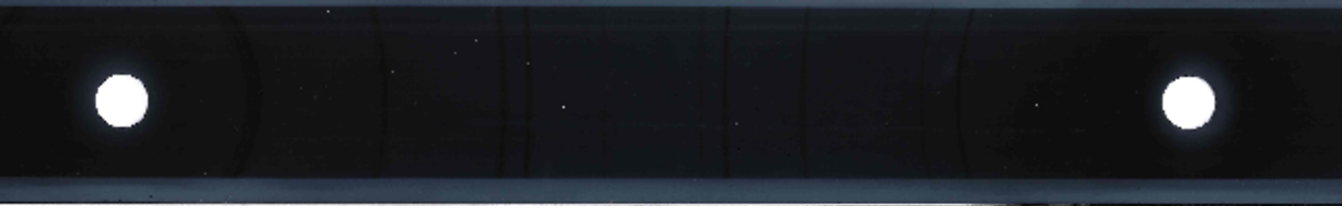
\includegraphics[scale=0.5]{content/pics/Metall_film.pdf}
  \caption{Filmaufnahme der Metallprobe \enquote{Metall 3}. Der Winkel \SI{0}{\degree} liegt in der
  rechten, der Winkel \SI{180}{\degree} in der linken Stanzung}
  \label{Abb:Metall}
\end{figure}

\begin{table}[H]
  \centering
  \caption{Beugungsreflexe an der Metallprobe \enquote{Metall 3} und zugeordnete Millerindizes
  und Gitterkonstanten für das bcc und das fcc-Gitter.}
  \label{Tab:Metall}
  \begin{tabular}{c || c c c c c|c c c c c}
    \toprule
    Winkel / ° &
    $n_{\text{bcc}}^{2}$ &
    $h_{\text{bcc}}$ &
    $k_{\text{bcc}}$ &
    $l_{\text{bcc}}$ &
    $a_{\text{bcc}}$ / pm &
    $n_{\text{fcc}}^{2}$ &
    $h_{\text{fcc}}$ &
    $k_{\text{fcc}}$ &
    $l_{\text{fcc}}$ &
    $a_{\text{fcc}}$ / pm \\
    \midrule
    40.35 & 2 & 1 & 1 & 0 & 315.92 & 3 & 1 & 1 & 1 & 386.92 \\
46.32 & 4 & 2 & 0 & 0 & 391.83 & 4 & 2 & 0 & 0 & 391.83 \\
65.61 & 6 & 2 & 1 & 1 & 348.32 & 8 & 2 & 2 & 0 & 402.21 \\
79.65 & 8 & 2 & 2 & 0 & 340.27 & 11 & 3 & 1 & 1 & 399.00 \\
112.63 & 10 & 3 & 1 & 0 & 292.80 & 12 & 2 & 2 & 2 & 320.75 \\
116.84 & 12 & 2 & 2 & 2 & 313.29 & 16 & 4 & 0 & 0 & 361.75 \\
136.84 & 14 & 3 & 2 & 1 & 310.01 & 19 & 3 & 3 & 1 & 361.15 \\
158.60 & 16 & 4 & 0 & 0 & 313.64 & 20 & 4 & 2 & 0 & 350.66 \\

    \bottomrule
  \end{tabular}
\end{table}

% \begin{table}[H]
%   \centering
%   \caption{Beugungsreflexe an der Metallprobe und zugeordnete Millerindizes
%   und Gitterkonstanten für das bcc-Gitter.}
%   \label{Tab:Metall_bcc}
%   \begin{tabular}{c || c c c c c}
%     \toprule
%     Winkel / ° &
%     $n_{\text{bcc}}^{2}$ &
%     $h_{\text{bcc}}$ &
%     $k_{\text{bcc}}$ &
%     $l_{\text{bcc}}$ &
%     $a_{\text{bcc}}$ / pm \\
%     \midrule
%     40.35 & 2 & 1 & 1 & 0 & 315.92 \\
46.32 & 4 & 2 & 0 & 0 & 391.83 \\
65.61 & 6 & 2 & 1 & 1 & 348.32 \\
79.65 & 8 & 2 & 2 & 0 & 340.27 \\
83.86 & 10 & 3 & 1 & 0 & 364.61 \\
100.00 & 12 & 2 & 2 & 2 & 348.41 \\
112.63 & 14 & 3 & 2 & 1 & 346.45 \\
116.84 & 16 & 4 & 0 & 0 & 361.75 \\
136.84 & 18 & 4 & 1 & 1 & 351.52 \\
158.60 & 20 & 4 & 2 & 0 & 350.66 \\

%     \bottomrule
%   \end{tabular}
% \end{table}
%
% \begin{table}[H]
%   \centering
%   \caption{Beugungsreflexe an der Metallprobe und zugeordnete Millerindizes
%   und Gitterkonstanten für das fcc-Gitter.}
%   \label{Tab:Metall_fcc}
%   \begin{tabular}{c || c c c c c}
%     \toprule
%     Winkel / ° &
%     $n_{\text{fcc}}^{2}$ &
%     $h_{\text{fcc}}$ &
%     $k_{\text{fcc}}$ &
%     $l_{\text{fcc}}$ &
%     $a_{\text{fcc}}$ / pm \\
%     \midrule
%     40.35 & 3 & 1 & 1 & 1 & 386.92 \\
46.32 & 4 & 2 & 0 & 0 & 391.83 \\
65.61 & 8 & 2 & 2 & 0 & 402.21 \\
79.65 & 11 & 3 & 1 & 1 & 399.00 \\
83.86 & 12 & 2 & 2 & 2 & 399.41 \\
100.00 & 16 & 4 & 0 & 0 & 402.31 \\
112.63 & 19 & 3 & 3 & 1 & 403.60 \\
116.84 & 20 & 4 & 2 & 0 & 404.45 \\
136.84 & 24 & 4 & 2 & 2 & 405.90 \\
158.60 & 27 & 5 & 1 & 1 & 407.43 \\

%     \bottomrule
%   \end{tabular}
% \end{table}
%
% \begin{table}[H]
%   \centering
%   \caption{Beugungsreflexe an der Metallprobe und zugeordnete Millerindizes
%   und Gitterkonstanten für die Diamantstruktur.}
%   \label{Tab:Metall_Dia}
%   \begin{tabular}{c || c c c c c}
%     \toprule
%     Winkel / ° &
%     $n_{\text{Diamant}}^{2}$ &
%     $h_{\text{Diamant}}$ &
%     $k_{\text{Diamant}}$ &
%     $l_{\text{Diamant}}$ &
%     $a_{\text{Diamant}}$ / pm \\
%     \midrule
%     40.35 & 1 & 1 & 0 & 0 & 223.39 \\
46.32 & 3 & 1 & 1 & 1 & 339.33 \\
65.61 & 5 & 2 & 1 & 0 & 317.97 \\
79.65 & 6 & 2 & 1 & 1 & 294.68 \\
83.86 & 8 & 2 & 2 & 0 & 326.12 \\
100.00 & 9 & 2 & 2 & 1 & 301.73 \\
112.63 & 10 & 3 & 1 & 0 & 292.80 \\
116.84 & 11 & 3 & 1 & 1 & 299.95 \\
136.84 & 13 & 3 & 2 & 0 & 298.73 \\
158.60 & 16 & 4 & 0 & 0 & 313.64 \\

%     \bottomrule
%   \end{tabular}
% \end{table}

\begin{figure}[h!]
  \centering
  \subcaptionbox{Zur Position in \autoref{Abb:Metall} korrespondierende
  Peaks. \label{Abb:Metall_Peaks}}[0.45\textwidth]{
  \centering
  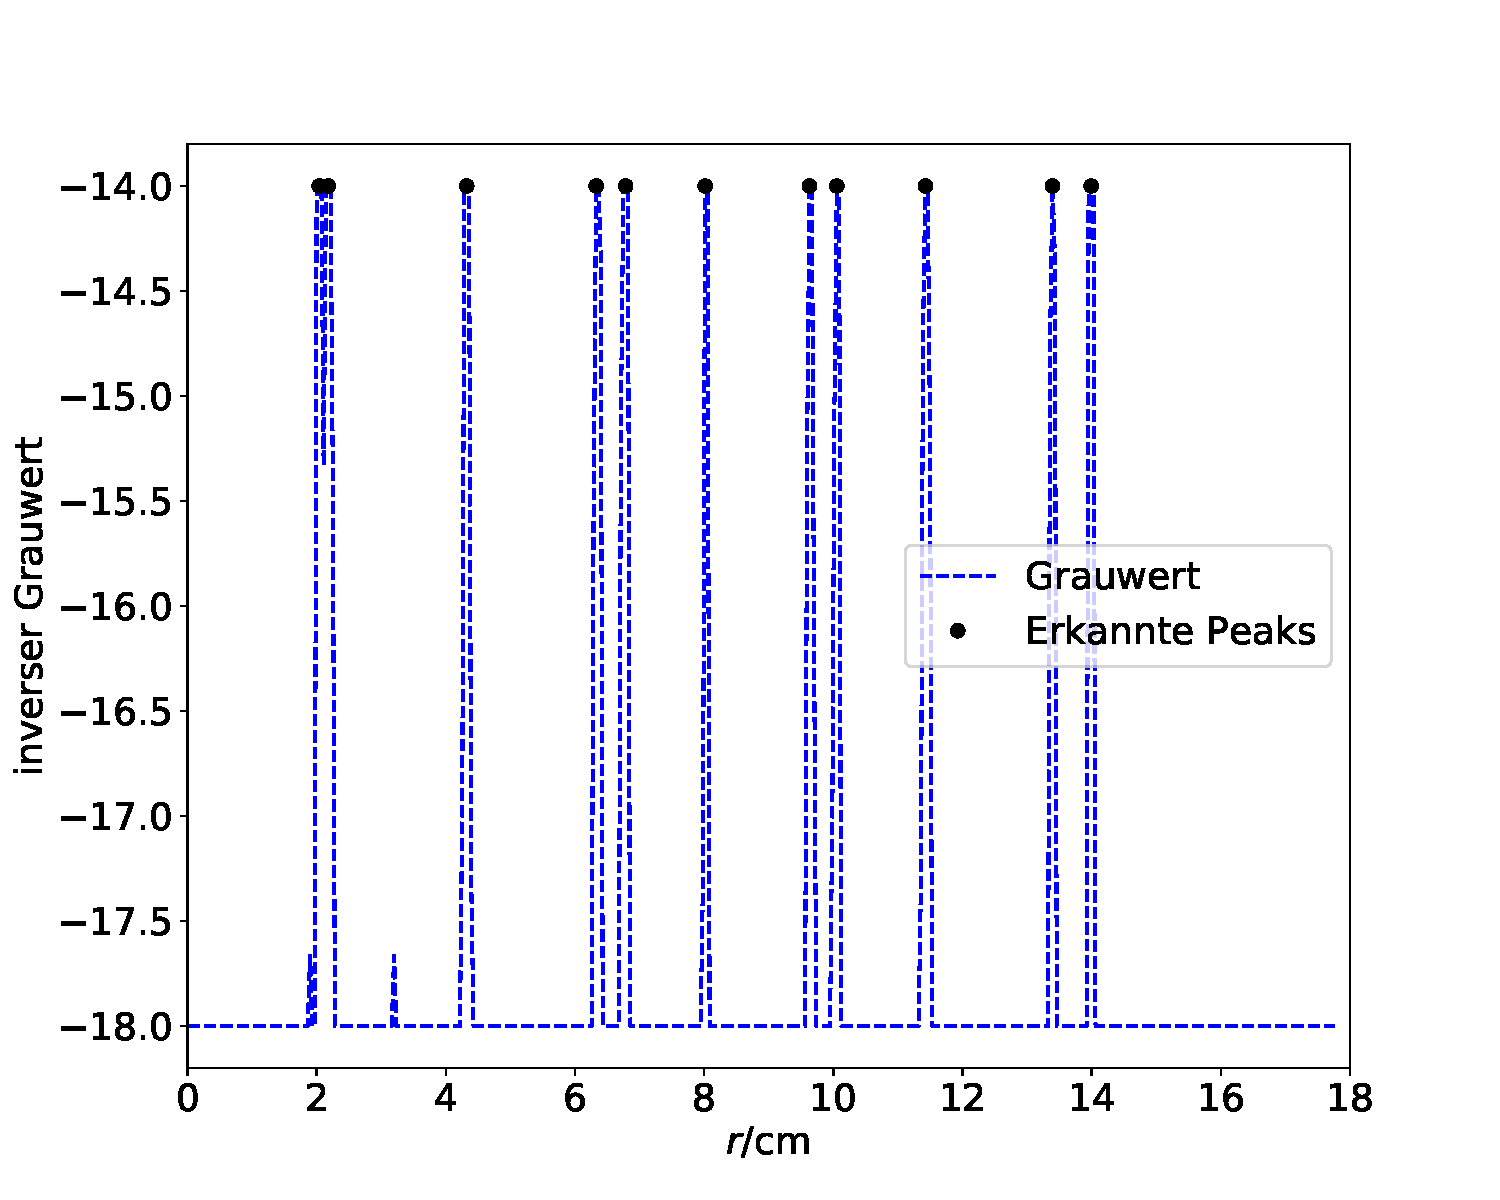
\includegraphics[width=0.45\textwidth]{Auswertung/Grafiken/Metall_Peaks.pdf}
  }
  \subcaptionbox{Gitterkonstante mit Ausgleichsrechnung. Die Position der Peaks wurde
  dafür invertiert, die einzellnen Hypothesen sind untenstehend
  in eigenen Grafiken zu finden. \label{Abb:Metall_a}}[0.45\textwidth]{
  \centering
  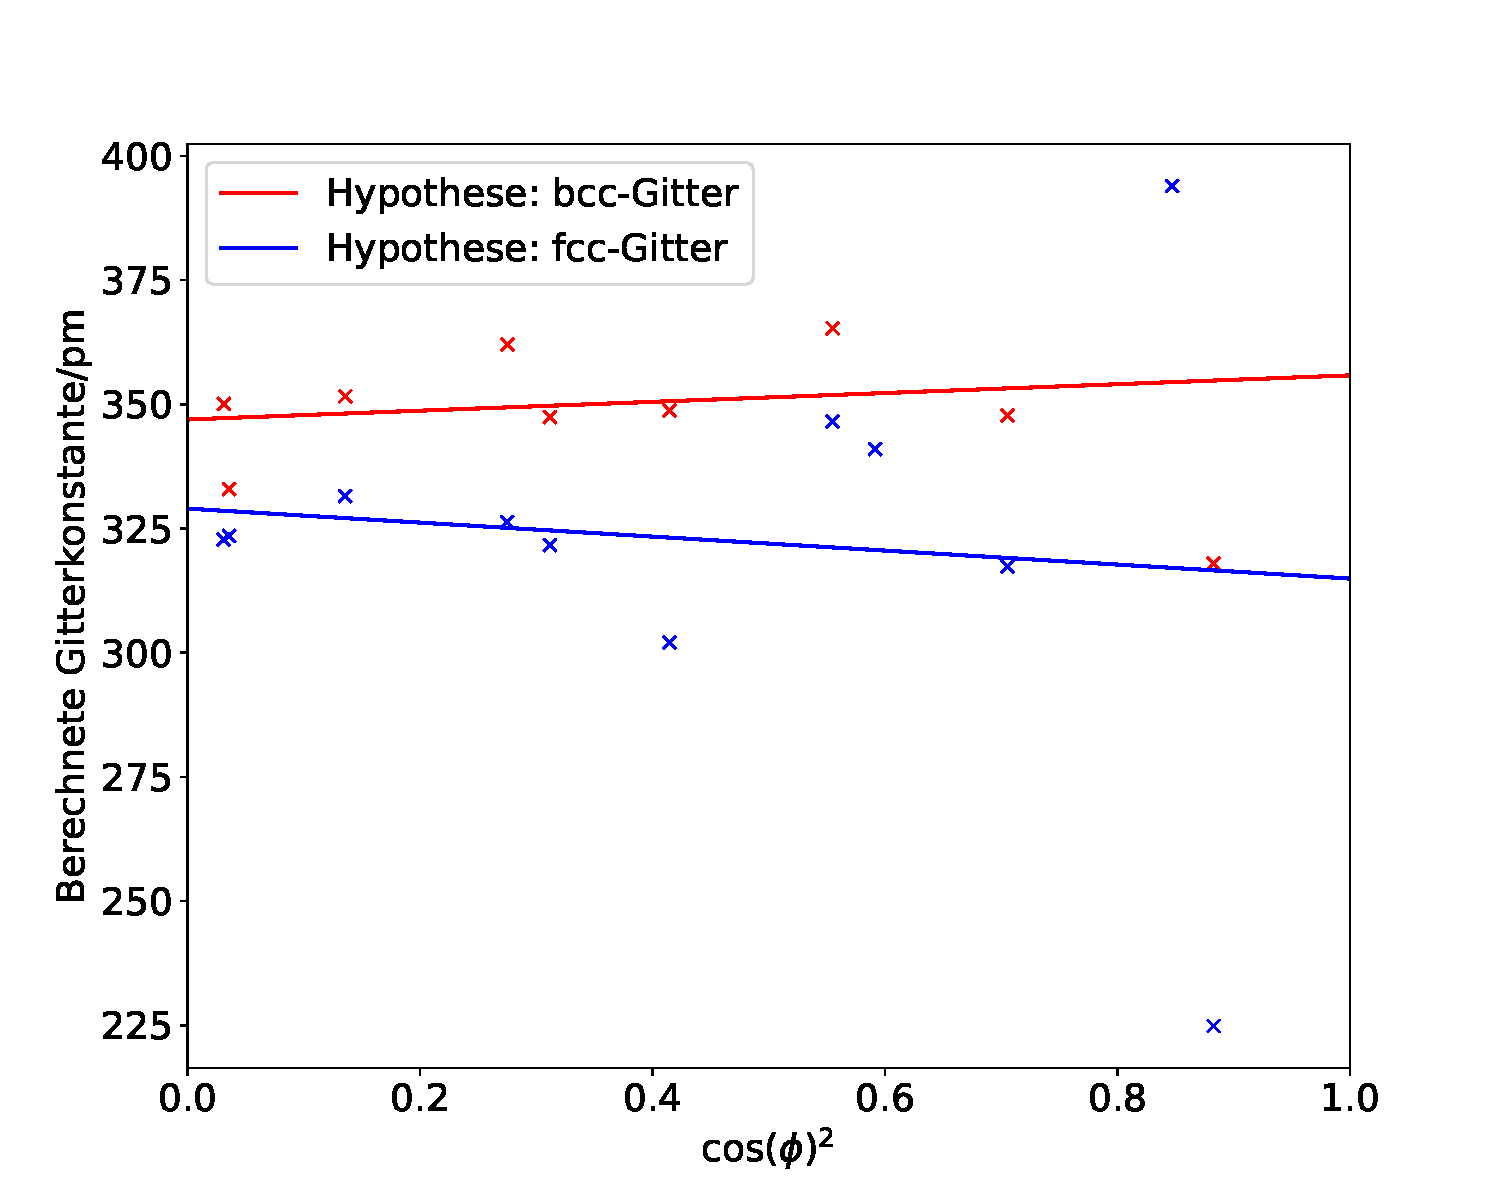
\includegraphics[width=0.45\textwidth]{Auswertung/Grafiken/Metall_Ausgleichsrechnung.pdf}
  }\\
  \label{Abb:Metall_Plots}
  \caption{Grafiken für die Metallprobe \enquote{Metall 3}.}
\end{figure}

\begin{figure}[p]
  \centering
  \subcaptionbox{Gitterkonstante mit Ausgleichsrechnung für die fcc-Struktur.
  \label{Abb:Metall_fcc}}[0.7\textwidth]{
  \centering
  \includegraphics[width=0.7\textwidth]{Auswertung/Grafiken/Metall_fcc_Ausgleichsrechnung.pdf}
  }\\
  \subcaptionbox{Gitterkonstante mit Ausgleichsrechnung für die bcc-Struktur.
  \label{Abb:Metall_bcc}}[0.7\textwidth]{
  \centering
  \includegraphics[width=0.7\textwidth]{Auswertung/Grafiken/Metall_bcc_Ausgleichsrechnung.pdf}
  }\\
  \label{Abb:Metall_Plots_a}
  \caption{Einzelgrafiken für die Metallprobe \enquote{Metall 3}.}
\end{figure}

\begin{table}[H]
  \centering
  \caption{Parameter der Ausgleichsrechnung für die Metallprobe \enquote{Metall 3}.}
  \label{Tab:Metall_Regression}
  \begin{tabular}{c | c c }
    \toprule
    Gittertyp &
    $m$ / $\frac{\mathrm{pm}}{1}$ &
    $n$ / pm \\
    \midrule
    bcc & \num{-2(23)} & \num{353(13)} \\
    fcc & \num{-20(4)} & \num{409.6(20)} \\
    % Diamant & \num{20(40)} & \num{285(22)} \\
    \bottomrule
  \end{tabular}
\end{table}

\subsection{Salzprobe}
Der Ausschnitt zwischen den Stanzungen des Films ist in \autoref{Abb:Salz}
zu sehen, die ausgelesenen Reflexe mit den zugeordneten Millerindizes für die
Hypothesen verschiedener kubischer Gitterstruktur finden sich mit den entsprechend
berechneten Gitterkonstanten in \autoref{Tab:Salza} und \autoref{Tab:Salzb}.
Zusätzlich sind in \autoref{Abb:Salz_Peaks} die ausgelesenen Peaks eingezeichnet.
Aufgrund der starken Belichtung des Films und der zusätzlichen Verunreinigung durch Streulicht
war es nicht möglich, helle und dunkle Reflexe zu trennen.
Wider ist eine Ausgleichsrechnung mit einer linearen Funktion für beide Gittertypen in
\autoref{Abb:Salz_a} gezeigt, die einzellnen Grafiken finden sich in \autoref{Abb:Salz_ZnS},
\autoref{Abb:Salz_CsCl}, \autoref{Abb:Salz_F} und \autoref{Abb:Salz_NaCl}. Die bestimmte Steigung $m$ und der y-Achsenabschnitt $n$
finden sich in Tabelle \autoref{Tab:Salz_Regression}.
Es zeigt sich, dass die Zinkblende-Typ Hypothese mit einer Gitterkonstante von
\SI{552(4)}{\pico\metre} den geringsten Fehler aufweist.

\begin{figure}
  \centering
  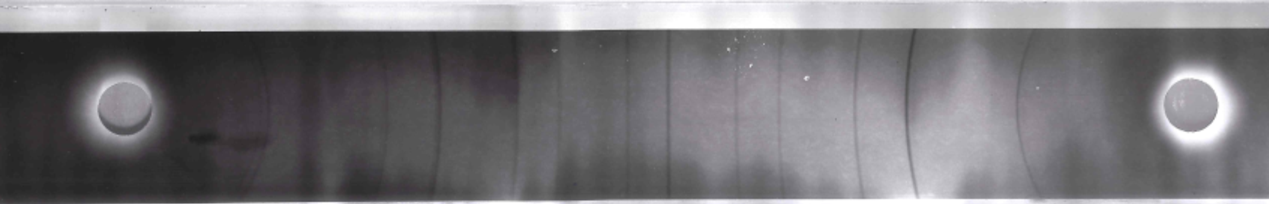
\includegraphics[scale=0.5]{content/pics/Salz_film.pdf}
  \caption{Filmaufnahme der Salzprobe \enquote{Salz 2}. Der Winkel \SI{0}{\degree} liegt in der
  rechten, der Winkel \SI{180}{\degree} in der linken Stanzung. Es ist ein
  deutlicher Verlauf von dunkel (links) nach hell (rechts) zu erkennen, der durch
  einfallendes Streulicht verursacht wurde.}
  \label{Abb:Salz}
\end{figure}

\begin{table}[H]
  \centering
  \caption{Beugungsreflexe an der Salzprobe \enquote{Salz 2} und zugeordnete Millerindizes und Gitterkonstanten
  für Zinkblende- und Cäsiumchlorid-Struktur}
  \label{Tab:Salza}
  \begin{tabular}{c || c c c c c|c c c c c}
    \toprule
    Winkel / ° &
    $n_{\text{ZnS}}^{2}$ &
    $h_{\text{ZnS}}$ &
    $k_{\text{ZnS}}$ &
    $l_{\text{ZnS}}$ &
    $a_{\text{ZnS}}$ / pm &
    $n_{\text{CsCl}}^{2}$ &
    $h_{\text{CsCl}}$ &
    $k_{\text{CsCl}}$ &
    $l_{\text{CsCl}}$ &
    $a_{\text{CsCl}}$ / pm \\
    \midrule
    30.82 & 1 & 1 & 0 & 0 & 289.98 & 6 & 2 & 1 & 1 & 710.29 \\
49.38 & 2 & 1 & 1 & 0 & 260.86 & 8 & 2 & 2 & 0 & 521.73 \\
58.13 & 9 & 2 & 2 & 1 & 475.77 & 10 & 3 & 1 & 0 & 501.51 \\
70.74 & 9 & 3 & 0 & 0 & 399.31 & 16 & 4 & 0 & 0 & 532.41 \\
78.09 & 12 & 2 & 2 & 2 & 423.68 & 22 & 3 & 3 & 2 & 573.66 \\
89.30 & 14 & 3 & 2 & 1 & 410.21 & 24 & 4 & 2 & 2 & 537.09 \\
96.30 & 17 & 4 & 1 & 0 & 426.45 & 26 & 4 & 3 & 1 & 527.39 \\
107.86 & 17 & 3 & 2 & 2 & 393.01 & 30 & 5 & 2 & 1 & 522.09 \\
114.51 & 18 & 4 & 1 & 1 & 388.63 & 32 & 4 & 4 & 0 & 518.18 \\
127.82 & 18 & 3 & 3 & 0 & 363.97 & 34 & 5 & 3 & 0 & 500.22 \\
136.58 & 19 & 3 & 3 & 1 & 361.48 & 38 & 6 & 1 & 1 & 511.21 \\
157.24 & 22 & 3 & 3 & 2 & 368.63 & 40 & 6 & 2 & 0 & 497.06 \\

    \bottomrule
  \end{tabular}
\end{table}

\begin{table}[H]
  \centering
  \caption{Beugungsreflexe an der Salzprobe \enquote{Salz 2} und zugeordnete Millerindizes und Gitterkonstanten
  für NaCl- und Flourid-Struktur.}
  \label{Tab:Salzb}
  \begin{tabular}{c || c c c c c|c c c c c}
    \toprule
    Winkel / ° &
    $n_{\text{NaCl}}^{2}$ &
    $h_{\text{NaCl}}$ &
    $k_{\text{NaCl}}$ &
    $l_{\text{NaCl}}$ &
    $a_{\text{NaCl}}$ / pm &
    $n_{\text{F}}^{2}$ &
    $h_{\text{F}}$ &
    $k_{\text{F}}$ &
    $l_{\text{F}}$ &
    $a_{\text{F}}$ / pm \\
    \midrule
    30.82 & 2 & 1 & 1 & 0 & 410.09 & 3 & 1 & 1 & 1 & 502.25 \\
49.38 & 3 & 1 & 1 & 1 & 319.49 & 4 & 2 & 0 & 0 & 368.92 \\
58.13 & 4 & 2 & 0 & 0 & 317.18 & 8 & 2 & 2 & 0 & 448.56 \\
70.74 & 5 & 2 & 1 & 0 & 297.63 & 11 & 3 & 1 & 1 & 441.45 \\
78.09 & 6 & 2 & 1 & 1 & 299.58 & 12 & 2 & 2 & 2 & 423.68 \\
89.30 & 8 & 2 & 2 & 0 & 310.09 & 16 & 4 & 0 & 0 & 438.53 \\
96.30 & 9 & 2 & 2 & 1 & 310.29 & 19 & 3 & 3 & 1 & 450.84 \\
107.86 & 10 & 3 & 1 & 0 & 301.43 & 20 & 4 & 2 & 0 & 426.28 \\
114.51 & 11 & 3 & 1 & 1 & 303.81 & 24 & 4 & 2 & 2 & 448.75 \\
127.82 & 12 & 2 & 2 & 2 & 297.18 & 27 & 5 & 1 & 1 & 445.77 \\
136.58 & 13 & 3 & 2 & 0 & 299.01 & 32 & 4 & 4 & 0 & 469.12 \\
157.24 & 14 & 3 & 2 & 1 & 294.06 & 35 & 5 & 3 & 1 & 464.96 \\

    \bottomrule
  \end{tabular}
\end{table}

\begin{figure}[h!]
  \centering
  \subcaptionbox{Zur Position in \autoref{Abb:Salz} korrespondierende
  Peaks. \label{Abb:Salz_Peaks}}[0.45\textwidth]{
  \centering
  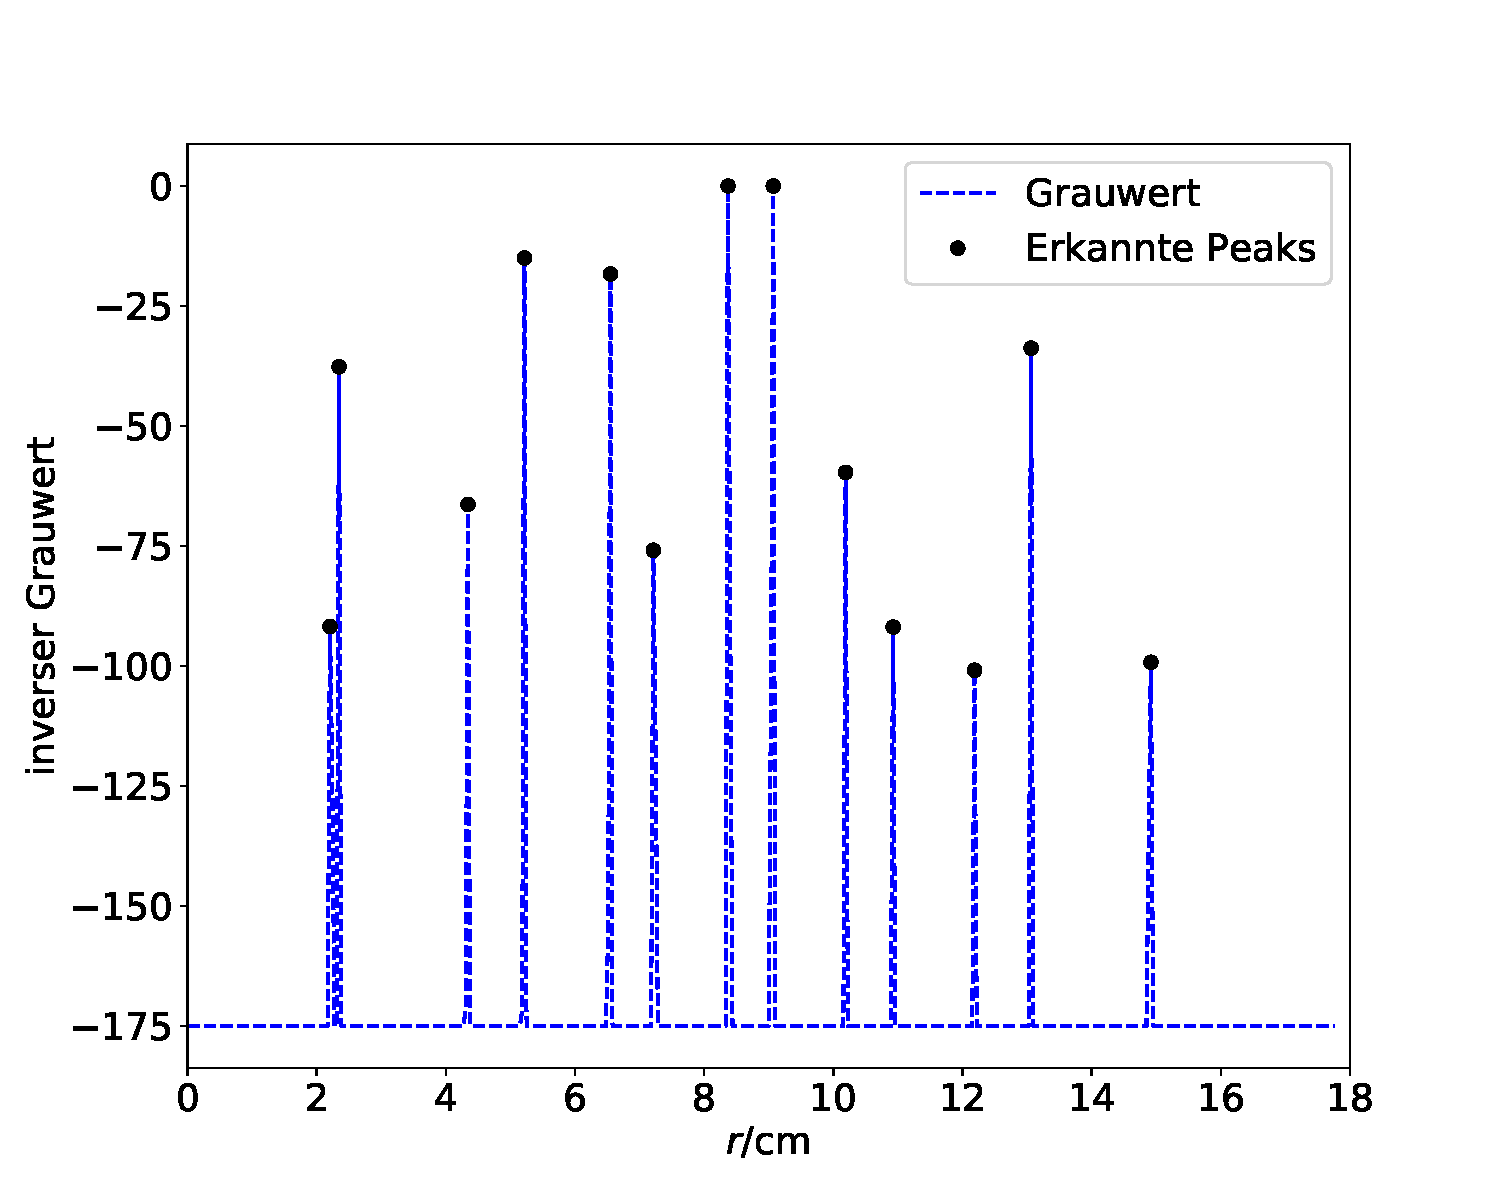
\includegraphics[width=0.45\textwidth]{Auswertung/Grafiken/Salt_Peaks.pdf}
  }
  \subcaptionbox{Gitterkonstante mit Ausgleichsrechnung. Die Position der Peaks wurde
  dafür invertiert, die einzellnen Hypothesen sind untenstehend in eigenen Grafiken zu finden.
  \label{Abb:Salz_a}}[0.45\textwidth]{
  \centering
  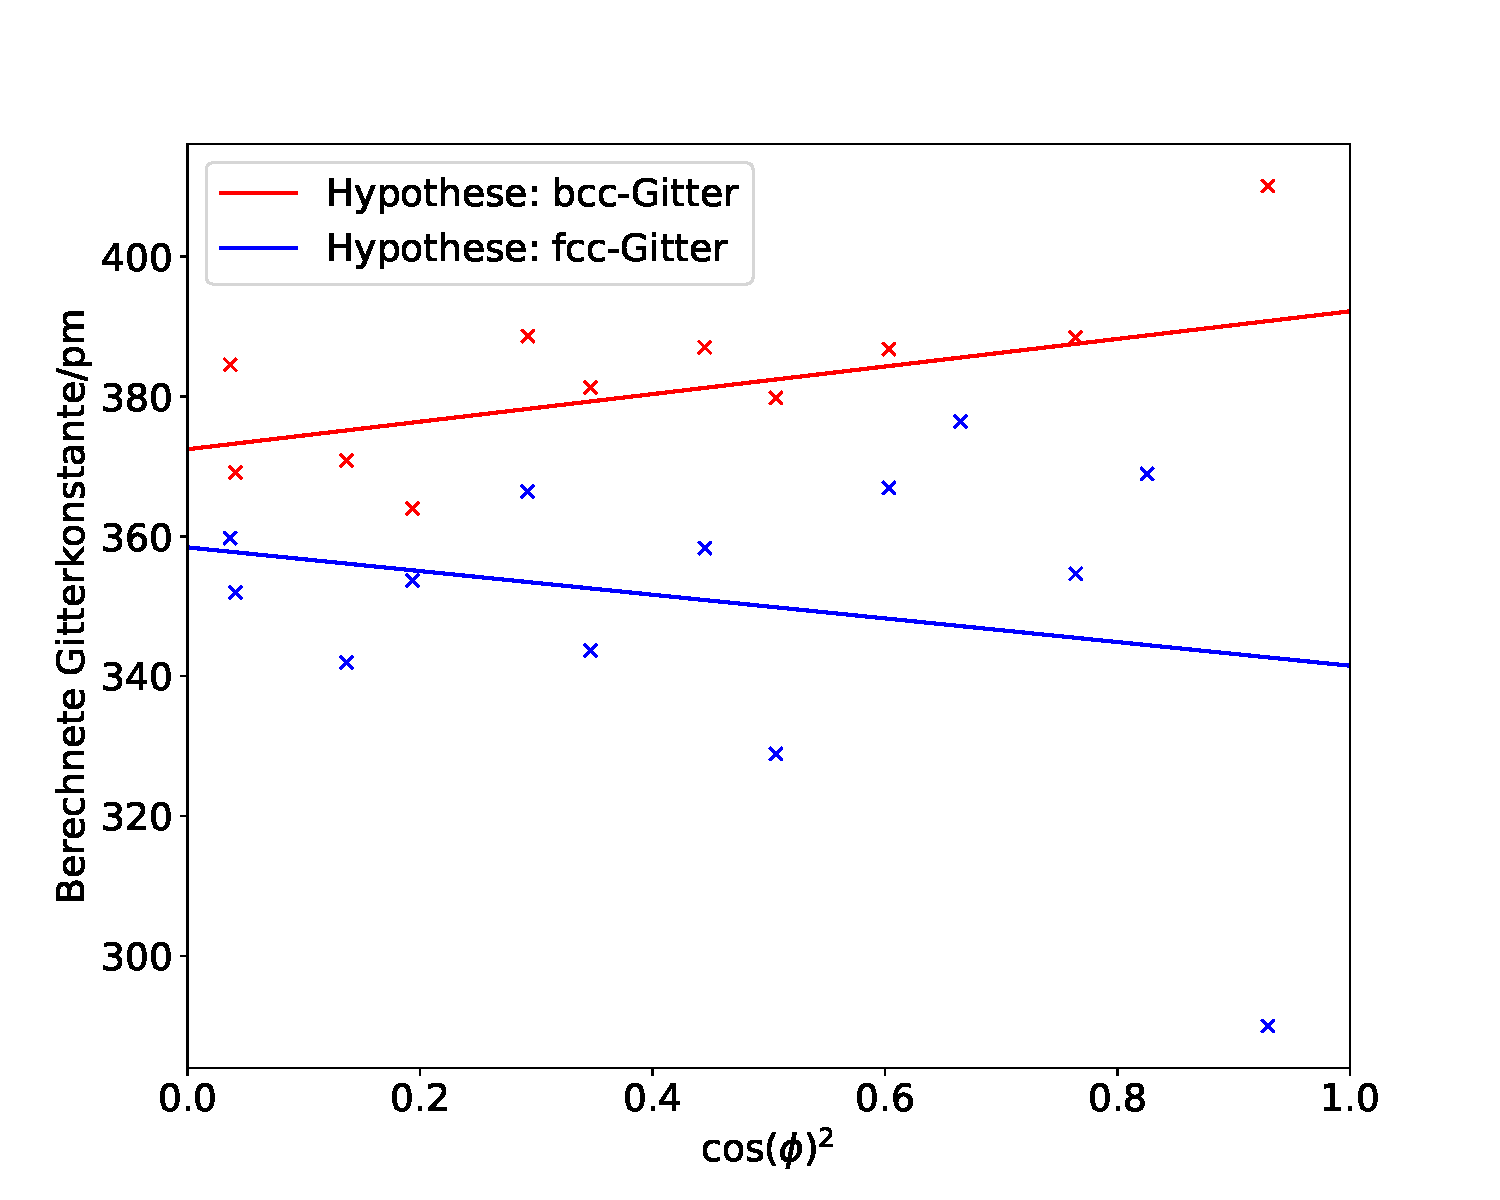
\includegraphics[width=0.45\textwidth]{Auswertung/Grafiken/Salt_Ausgleichsrechnung.pdf}
  }\\
  \label{Abb:Salz_Plots}
  \caption{Grafiken für die Salzprobe \enquote{Salz 2}.}
\end{figure}

\begin{figure}[h!]
  \centering
  \subcaptionbox{Gitterkonstante mit Ausgleichsrechnung für die Zinkblende-Struktur.
  \label{Abb:Salz_ZnS}}[0.7\textwidth]{
  \centering
  \includegraphics[width=0.7\textwidth]{Auswertung/Grafiken/Salt_ZnS_Ausgleichsrechnung.pdf}
  }\\
  \subcaptionbox{Gitterkonstante mit Ausgleichsrechnung für die Cäsiumchlorid-Struktur.
  \label{Abb:Salz_CsCl}}[0.7\textwidth]{
  \centering
  \includegraphics[width=0.7\textwidth]{Auswertung/Grafiken/Salt_CsCl_Ausgleichsrechnung.pdf}
  }\\
  \label{Abb:Salz_Plotsa}
  \caption{Einzelgrafiken für die Salzprobe \enquote{Salz 2}.}
\end{figure}

\begin{figure}[h!]
  \centering
  \subcaptionbox{Gitterkonstante mit Ausgleichsrechnung für die NaCl-Struktur.
  \label{Abb:Salz_NaCl}}[0.7\textwidth]{
  \centering
  \includegraphics[width=0.7\textwidth]{Auswertung/Grafiken/Salt_NaCl_Ausgleichsrechnung.pdf}
  }\\
  \subcaptionbox{Gitterkonstante mit Ausgleichsrechnung für die Flourit-Struktur.
  \label{Abb:Salz_F}}[0.7\textwidth]{
  \centering
  \includegraphics[width=0.7\textwidth]{Auswertung/Grafiken/Salt_F_Ausgleichsrechnung.pdf}
  }\\
  \label{Abb:Salz_Plotsn}
  \caption{Einzelgrafiken für die Salzprobe \enquote{Salz 2}.}
\end{figure}

\begin{table}[H]
  \centering
  \caption{Parameter der Ausgleichsrechnung für die Salzprobe \enquote{Salz 2}.}
  \label{Tab:Salz_Regression}
  \begin{tabular}{c | c c }
    \toprule
    Gittertyp &
    $m$ / $\frac{\mathrm{pm}}{1}$ &
    $n$ / pm \\
    \midrule
    ZnS & \num{-40(6)} & \num{552(4)} \\
    CsCl & \num{4(11)} & \num{383(6)} \\
    NaCl & \num{71(27)} & \num{280(15)} \\
    F & \num{-21(34)} & \num{454(19)} \\
    \bottomrule
  \end{tabular}
\end{table}

\section{Diskussion}
Die Metallprobe zeigt gut auszuwertende Ergebnisse. Aufgrund der guten Abschirmung
und der geringeren Belichtungsdauer als bei der Salzprobe können alle Reflexe gut
beobachtet werden. Mit einer Gitterkonstante von \SI{409.6(20)}{\pico\metre}
bewegt sich das Analyseergebnis in einem für Metalle typischen Bereich.
Insbesondere der sehr geringe Fehler weißt auf eine genaue Bestimmung hin.
Innerhalb der Fehlertoleranz des Messwertes liegt das in fcc-Struktur kristallisierende
Silber mit einer Gitterkonstante von \SI{409}{\pico\metre}\cite{AM}. Die Zuordnung erscheint
auch wegen der gräulich-silbrigen Erscheinung der Probe als sinnvoll.\\
Auch die saline Probe liegt mit einer Gitterkonstante von \SI{552(4)}{\pico\metre}
in einer passenden Größenordnung. Insbesondere der Namensgeber der ZnS-Struktur,
das Znksulfid oder auch Zinkblende, liegt mit einer Gitterkonstante von
\SI{541}{\pico\metre}\cite{AM} innerhalb einer $3\sigma$-Umgebung des bestimmten Wertes.
Hierbei ist auch das Aussehen der Probe als weißes Pulver passend.
Problematisch gestalltete sich bei der salinen Probe die starke Verunreinigung
durch eingedrungenes Steulicht. Dadurch wird insbesondere die Erkennung schwacher
Reflexe schwierig und die Gefahr, schwache Refelexe zu übersehen steigt.
Für ein sichereres Ergebnis ist die Messung daher mit verbesserter Streulichtabschirmung
zu wiederholen.
